\section{Metodologia de Desenvolvimento}
\label{sec:desenvolvimento}

Esta Seção descreve o método de desenvolvimento da ferramenta Cupper.
Os itens estão diretamente relacionados com as metodologias, técnicas e
práticas utilizadas na Engenharia de Software, tais como ciclo de
desenvolvimento, testes, integração contínua, qualidade de código, etc.
Todos os itens utilizados fazem parte do conhecimento adquirido durante
o curso.

Como será observado nas subseções, as práticas e técnicas são provenientes
das Metodologias Ágeis. A motivação para a utilização da abordagem
ágil é a familiaridade e experiência dos desenvolvedores deste trabalho.

\subsection{Métodos Base}
\label{sec:metodo_base}

Segundo~\citeonline{gutierrez:2009} o método \textit{Scrum} representa um trabalho
em equipe no qual todos os integrantes e envolvidos trabalham para alcançar
o mesmo objetivo, alinhando as mudanças e compartilhando os problemas para que
todos caminhem para a mesma direção. O mesmo autor descreve o método
\textit{Extreme Programming (XP)} como eficiente, flexível e de baixo risco para equipes
pequenas e médias que convivem com constante mudanças.

Ambos os métodos definem pepéis, práticas e modelos de ciclo de vida para
projetos de desenvolvimentos ágeis e serão utilizados como base para a definição
do método de desenvolvimento deste trabalho.

\subsection{Práticas e Técnicas}
\label{sec:praticas_tecnicas}

São definidas algumas práticas no método \textit{Scrum}~\cite{gutierrez:2009}. A lista a seguir
mostra as que serão utilizadas, bem como a descrição das adaptações para o trabalho:

\begin{itemize}
  \item \textit{\textbf{Sprint}}: ciclos onde são desenvolvidos os itens propóstos. Geralmente
    são intervalos de 2-4 semanas. Ao final de cada \textit{Sprint} é entregue uma porção 
    executável do \textit{software}. Neste trabalho será utilizado \textit{Sprints} com período
    de 2 semanas;
  \item \textbf{\textit{Product Backlog}}: o \textit{Product Backlog} contém dos os itens a serem
    desenvolvidos no projeto, sendo uma visão macro de tudo a ser feito.
    Com o auxilio da ferramenta Github, os itens dos \textit{backlogs} serão dispostos
    como \textit{issues};
\end{itemize}

O XP traz doze práticas essenciais~\cite{gutierrez:2009}. A lista a seguir
mostra as que serão utilizadas, bem como a descrição das adaptações para o trabalho:

\begin{itemize}
  \item \textbf{Teste}: são divididas em duas partes: teste de aceitação, elaboradas pelo cliente,
    e testes de unidade, elaboradas pelo programador. Será utilizado apenas os testes
    de unidade com a ferramenta RSpec.
  \item \textit{\textbf{Refactoring}}: consiste em simplificar a estrutura, mudar a organização do código,
    sem que altere o comportamento~\cite{beck:2000}. Neste trabalho será utilizado
    conforme as necessidades, sendo levado em consideração a import{\^a}ncia, impactos na
    arquitetura da ferramenta e a prioridade em relação aos outros itens da \textit{Sprint};
  \item \textbf{Integração Contínua}: o código deve ser integrado e testado constantemente
    após o desenvolvimento de novas características. Com o auxílio do serviço Travis CI,
    os \textit{Pull Requests} e \textit{Branchs} serão monitorados quanto a integridade dos testes. Apenas
    será integrado os códigos que não tenham falhado durante a inspeção do serviço
    de integração contínua;
  \item \textbf{Programação em Pares}: dois programadores utilizam o mesmo equipamento para
    o desenvolvimento, sendo assim o código está sempre sendo supervisionado por
    outro programador. Técnica utilizada apenas quando necessário, como em uma grande
    alteração da estrutura ou no funcionamento de algum módulo ou classe.
\end{itemize}

\subsection{Controle de Versão}
\label{sec:ctrl_versao}

Segundo~\citeonline{pressman:2009}, a área da engenharia de software responsável por
gerenciar e controlar mudanças em um software é a gerência de configuração de software.
Nela são definidas as principais atividades que lidam com a identificação de alterações
dos itens de trabalho, estabelecedo uma relação entre eles, definir o gerenciamento das
versões de trabalho, controlar e auditar as mudanças impostas.

As principais preocupações da gerência de configuração é~\cite{pressman:2009}:
\begin{enumerate}
  \item Estabelecer as versões estáveis do sistema ou componente conhecido
    como \textit{baseline};
  \item Possibilitar desfazer modificações no sistema, por conta de erros,
    rejeição do usuário, etc;
  \item Recuperar informações sobre quem e o que foi alterado no sistema e como
    essa alteração está ligada com as necessidades do projeto;
\end{enumerate}

Quanto as ferramentas de suporte a gerência de configuração, existem várias alternativas.
Dentre elas, como mapeado na Seção \ref{sec:supdev:git}, tem-se o Git que é responsável pelo
controle de versão do sistema. Nela é possível contornar as principais preocupações
descritas acima.

\citeonline{driessen:2010} apresenta um modelo de fluxo de desenvolvimento utilizando a
ferramenta Git. Nele são abordados as estratégias de controle de \textit{branchs} e
gerenciamento de \textit{release}. Com base nesse modelo, a Figura \ref{fig:ctrl_versao}
mostra o fluxo básico de desenvolvimento do Cupper.

\begin{figure}[H]
  \centering
  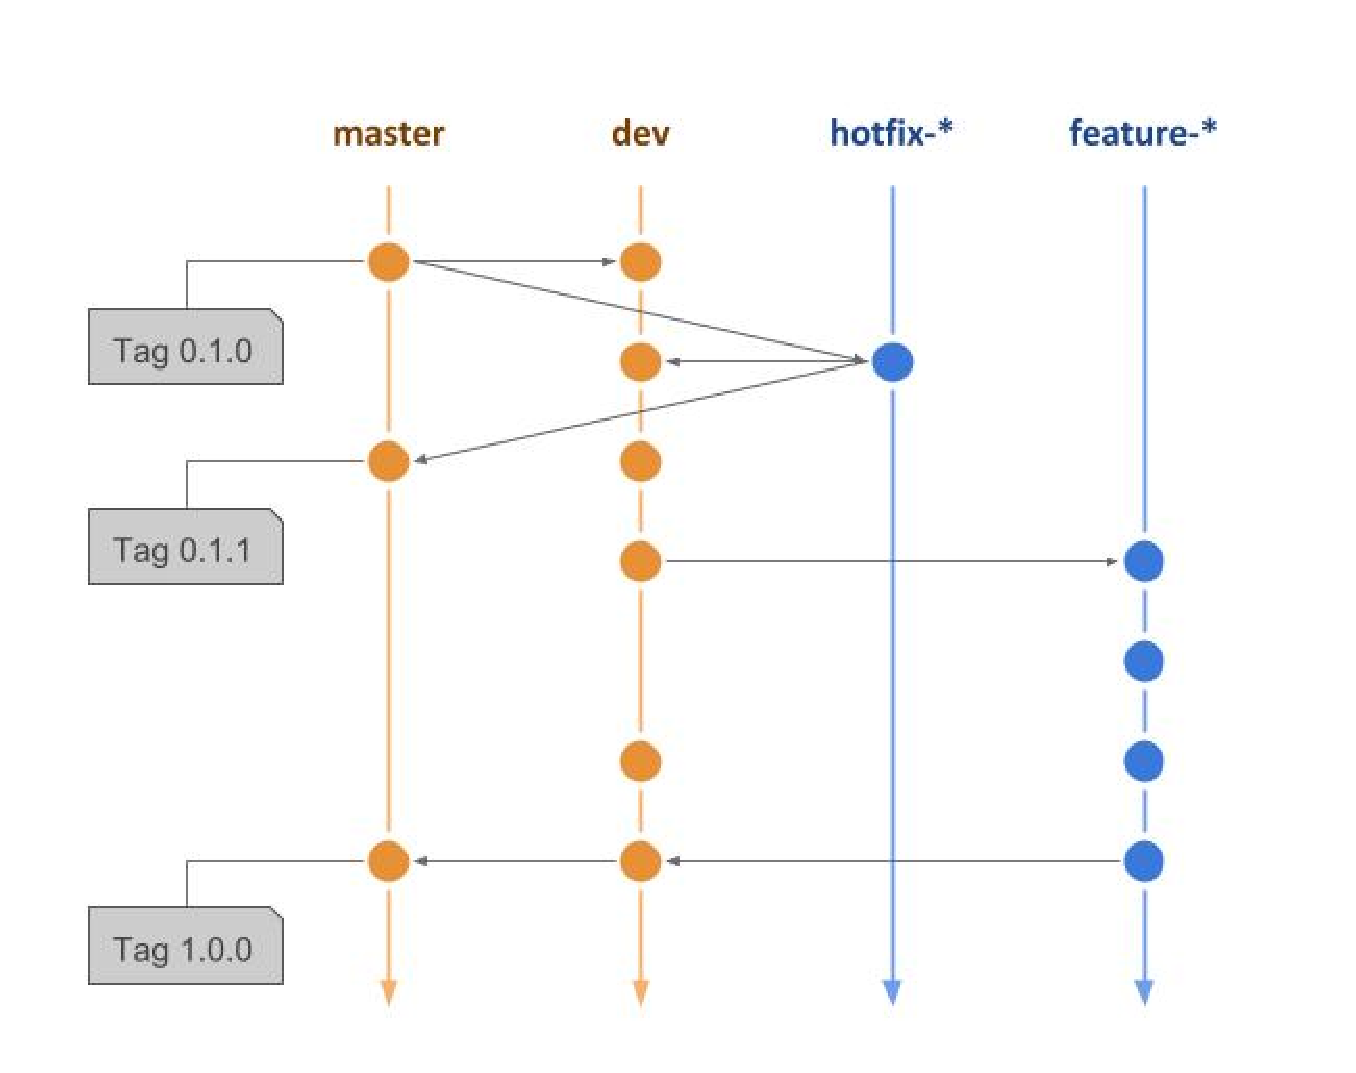
\includegraphics[width=0.8\textwidth]{figuras/controle_versao}
  \caption{Controle de versão do Cupper}
  \label{fig:ctrl_versao}
\end{figure}

Neste modelo, as principais \textit{branchs} tem o tempo de vida infinito, ou seja,
em nenhum momento são removidas do repositório remoto. São elas:

\begin{itemize}
  \item \textit{master}: reflete o estado de \lq\lq pronto para produção\rq\rq,
    ou seja, estabelece uma versão estável do sistema. Todo
    o trabalho realizado, em algum ponto do desenvolvimento
    deve ser integrado a esta \textit{branch};
  \item \textit{dev}: onde ocorre a integração de todos os componentes,
    funcionalidades e correções. Contém todos os itens mais
    recentes desenvolvidos e é considerado a versão instável
    do sistema, ou seja, pode conter comportamentos indesejados
    e \textit{bugs} desconhecidos.
\end{itemize}

Há também as \textit{branches} de suporte que tem o tempo de vida curto, ou seja,
assim que concluídas, devem ser removidas do repositório remoto. São
elas:

\begin{itemize}
  \item \textit{feature}: deve ser ramificada da \textit{branch dev} e
    integrada a \textit{branch dev} quando finalizada. Contém todos os
    novos itens desenvolvidos para a nova funcionalidade;
  \item \textit{hotfix}: deve ser ramificada da \textit{branch master} e
    integrada a \textit{branch dev} e \textit{master} quando finalizada. São
    as correções que são realizadas na versão estável do sistema, e geralmente
    são pontos críticos que devem ser corrigidos imediatamente. Quando finalizadas
    deve-se criar uma \textit{tag} da versão estável do sistema;
\end{itemize}
